\subsection{Ground station networks}

There are a lot of unknowns in this area. We don't know what network will be used, who will be participating or what kind of radio equipment will be used. A part of this project is to simulate some different possible ground networks to find how much data we can realistically download.  
Simulating a network consisting of NTNU and Aalborg University is interesting, since Aalborg University are the developers of the BlueBox satellite network. 

% Figurer
\begin{figure}
  \begin{center}
    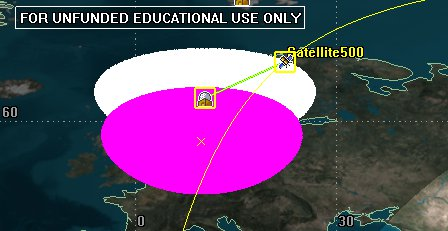
\includegraphics[width=0.7\textwidth]{Figures/range_ntnu_aalborg}
  \end{center}
  \caption{Ground station network: NTNU and Aalborg}
  \label{fig:range_ntnu_aalborg}
\end{figure}

\begin{figure}
  \begin{center}
    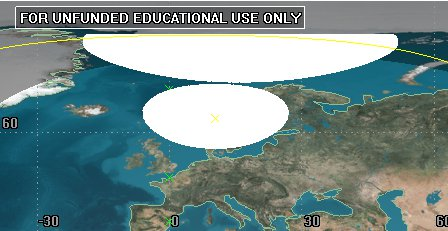
\includegraphics[width=0.7\textwidth]{Figures/range_ntnu_svalbard}
  \end{center}
  \caption{Ground station network: NTNU and UNIS}
  \label{fig:range_ntnu_unis}
\end{figure}

\begin{figure}
  \begin{center}
    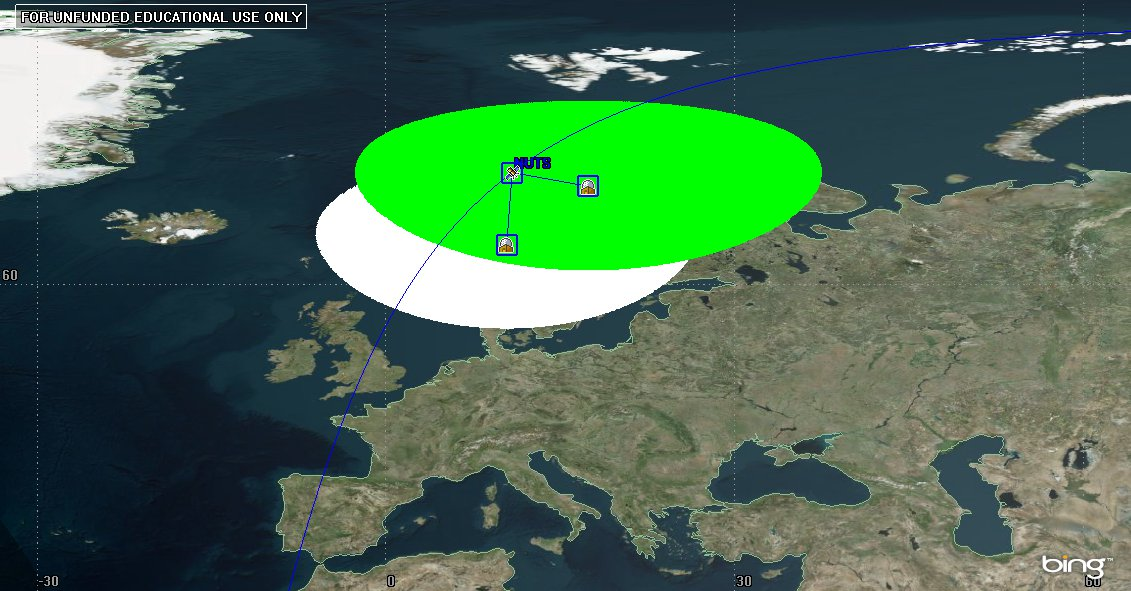
\includegraphics[width=0.7\textwidth]{Figures/range_ntnu_narvik}
  \end{center}
  \caption{Ground station network: NTNU and UiN}
  \label{fig:range_ntnu_unis}
\end{figure}


A ground station network consisting of NTNU and Aalborg University is not very efficent, see Fig. \ref{fig:range_ntnu_aalborg}. 
 


The results are summarised in Table \ref{tab:networks}.

\begin{table}
\begin{center}
\begin{tabular}{l | c c}
  Other locations & Time & Improvement \\
\hline \hline
  Aalborg & 790s &  50\% \\
\hline
  Longyearbyen & 1900s & 260\% \\
\hline
  Narvik & 900s & 73\%  \\
\end{tabular}
\end{center}
\caption{Some data}
\label{tab:networks}
\end{table}